\chapter{Introduction}\thispagestyle{empty} %chapter head
\graphicspath{{Chapter1/figures/}}
{\setstretch{1.5}
%--------------------------------------------------------------------------------------
Writing an introduction for a project report is an important step in setting the context and providing readers with a clear understanding of what the report will cover. Here’s a general guide on how to structure and write an effective introduction:

\section{Context and Background}
Begin by providing background information relevant to your project. Explain the broader context in which the project was undertaken. This might include industry trends, academic relevance, or organizational needs.
Example: "In recent years, the rapid advancement of technology has revolutionized the healthcare industry, making data management systems an essential component for modern hospitals. This project was undertaken to address the growing need for a secure and efficient database system at XYZ Hospital."
\section{Purpose of the Project}
Clearly state the purpose or objective of the project. This explains why the project was initiated and what it aims to achieve.
Example: "The primary objective of this project is to develop a database security framework that ensures the confidentiality, integrity, and availability of patient data at XYZ Hospital."
\section{ Scope of the Project}
Define the scope of the project. What aspects are included in the project, and what are the boundaries? This helps manage expectations and clarifies what the project will cover.
Example: "This report focuses on the design and implementation of security measures for the hospital's database system, including encryption, access control, and regular security audits. It does not cover the hospital's overall IT infrastructure."
\section{Significance of the Project}
Discuss the importance or significance of the project. Explain why the project is important and what impact it is expected to have.
Example: "With the increasing number of cyber threats targeting healthcare institutions, implementing a robust database security framework is crucial. This project not only enhances the security of sensitive patient data but also helps the hospital comply with regulatory requirements."


\begin{figure}[H]
\centering
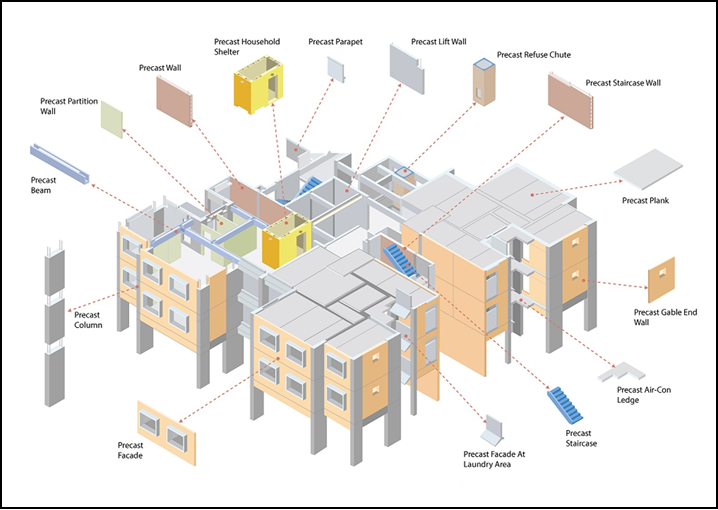
\includegraphics[width=\columnwidth, height =9cm]{Chapter1/figures/Precast1.png}
\caption{Prefabricated Building Systems}% \cite{PBS} }
\label{PBS}
\end {figure}

\section{System Architecture}
%Add classification picture here
Birkeland et.al \cite{birkeland1966connections} classified precast systems into large panel prefabrication systems, frame systems, shear walls, and mixed systems based on load carrying capacity of structures. Prefabrication systems are classified as open prefabrication systems (partial and full prefabrication), large panel prefabrication systems (staircase systems, balconies, precast floors and precast walls), and box type construction according to IS15916:2011\cite{standard15916criteria}, as shown in Figure \ref{PS}.

\begin{figure}[H]
\centering
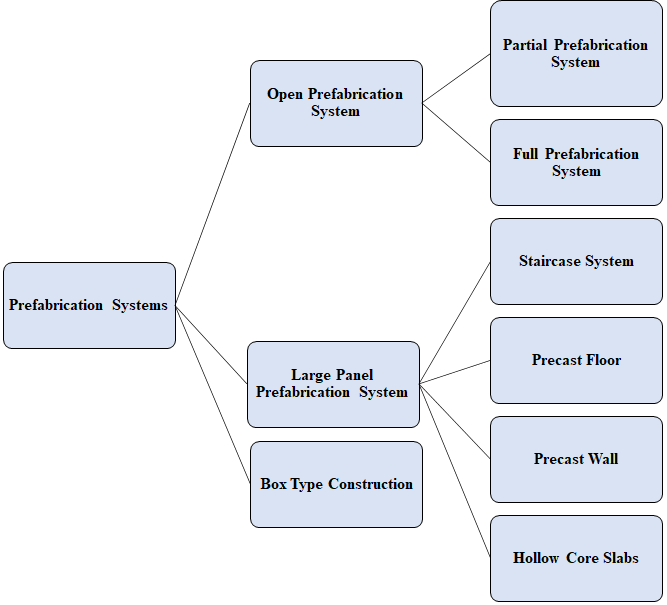
\includegraphics[width=0.7\columnwidth]{Chapter1/figures/PCClass.png}
\caption{Prefabrication Systems}
\label{PS}
\end {figure}


\section{Problem Statement}
The large panel system is made up of vertical and horizontally connected wall and floor concrete panels that enclose adequate spaces in a construction.
When horizontal floor/roof panels are properly connected, they function as diaphragms, transferring lateral loads to vertical elements. Wall panels are typically one storey high, with one-way or two-way slabs for floors and roofs.
 Figure \ref{LP} \cite{LPS} illustrates large wall panel systems.

\begin{figure}[H]
\centering
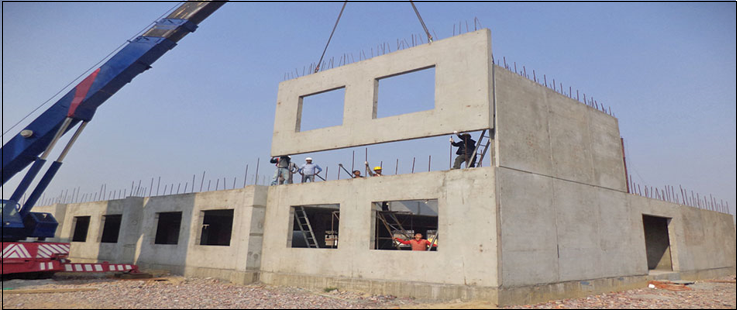
\includegraphics[width=0.7\columnwidth, height =5cm]{Chapter1/figures/LPS.png}
\caption{Large Panel Systems} %\cite{LPS}}
\label{LP}
\end {figure}





\section{Objectives}
Frame systems are structures with beams, columns, and slabs that can withstand both lateral and gravity loads, and they are widely used to overcome large moments produced by loading. As shown in Figure \ref{FS} \cite{FS}, frame systems are either rigid or braced, using linear or beam column components as part of the assembly.



\section{Applications}

The most critical research issue that concerns the precast industry is the development of a reliable and cost-effective technique for connecting prefabricated parts. The weak points in a prefabricated structural system are the locations of high stresses. Connection handling should be accomplished with the minimum amount of joint members possible, with the best possible transmissibility of existing forces and minimum secondary forces. According to the force transmission at the junction of structural components, joints are classified as compression joints, tensile joints, shear joints, flexure and torsional joints.


\section{ Structure of the Report}
Briefly outline the structure of the report. This gives readers a roadmap of what to expect in the following sections.
Example: "This report is organized as follows: Section 2 provides a literature review of current database security practices; Section 3 outlines the methodology used in the project; Section 4 discusses the implementation details; Section 5 presents the results and analysis; and Section 6 offers conclusions and recommendations."


\begin{table}[H]
\centering
\captionsetup{justification=centering}
\caption{Thesis Organization \&  Published and Submitted Papers}
%\resizebox{\textwidth}{!}{ 
\begin{tabular}{clcc}
\toprule
\textbf {Chapter}  & \textbf{Content}  & \textbf{Objective} & \textbf{Paper}  \\ 
\textbf { No.} & & &\\
\midrule
1 & Introduction &  &  I\\
\hline
%3 & Objectives& \\
%\hline
2 & Comparative Study of Prefabricated \\
& \& RC Multistoreyed residential building & 1 &  II\\
\hline
3  & Performance Evaluation of Precast\\
& Prestressed  Hollow Core Slabs & 2 &  III \&  IV\\
\hline
4  & Reliability Analysis of Precast \\
& Prestressed Hollow Core Slabs & 2 &  V\\
\hline
5  & AMPLE: An Approximate Modelling \\
& of Panel Link Elements & 3 &   VI \& VII\\
\hline
6  & Reliability Analysis for Bond Strength\\
& of Precast Panel Joints& 4&  VIII\\
\hline
7 & Conclusions & & \\
\bottomrule
\end{tabular}
\label{ContentL}
\end{table}

  
\textbf {Chapter 7 Conclusion} concludes the thesis by summarizing the results and future scope of research.







